%%%%%%%%%%%%%%%%%%%%%%%%%%%%%%%%%%%%%%%%%
% Professional Formal Letter
% LaTeX Template
% Version 2.0 (12/2/17)
%
% This template originates from:
% http://www.LaTeXTemplates.com
%
% Authors:
% Brian Moses
% Vel (vel@LaTeXTemplates.com)
%
% License:
% CC BY-NC-SA 3.0 (http://creativecommons.org/licenses/by-nc-sa/3.0/)
%
%%%%%%%%%%%%%%%%%%%%%%%%%%%%%%%%%%%%%%%%%

%----------------------------------------------------------------------------------------
%	PACKAGES AND OTHER DOCUMENT CONFIGURATIONS
%----------------------------------------------------------------------------------------

\documentclass[11pt, a4paper]{letter} % Set the font size (10pt, 11pt and 12pt) and paper size (letterpaper, a4paper, etc)


\usepackage{graphicx} % Required for including pictures

\usepackage[T1]{fontenc} % Output font encoding for international characters
\usepackage[utf8]{inputenc} % Required for inputting international characters
\usepackage{gfsdidot} % Use the GFS Didot font: http://www.tug.dk/FontCatalogue/gfsdidot/
\usepackage{microtype} % Improves typography

\usepackage{hyperref}
\hypersetup{hidelinks = true,}
\usepackage{xurl}
\usepackage{todonotes}

% %%%%%%%%%%%%%%%%%%%%%%%%%%%%%%%%%%%%%%%%%
% Professional Formal Letter
% Structure Specification File
% Version 1.0 (12/2/17)
%
% This file originates from:
% http://www.LaTeXTemplates.com
%
% Authors:	
% Brian Moses
% Vel (vel@LaTeXTemplates.com)
%
% License:
% CC BY-NC-SA 3.0 (http://creativecommons.org/licenses/by-nc-sa/3.0/)
%
%%%%%%%%%%%%%%%%%%%%%%%%%%%%%%%%%%%%%%%%%

%----------------------------------------------------------------------------------------
%	PACKAGES AND OTHER DOCUMENT CONFIGURATIONS
%----------------------------------------------------------------------------------------

\usepackage{graphicx} % Required for including pictures

\usepackage[T1]{fontenc} % Output font encoding for international characters
\usepackage[utf8]{inputenc} % Required for inputting international characters
\usepackage{gfsdidot} % Use the GFS Didot font: http://www.tug.dk/FontCatalogue/gfsdidot/
\usepackage{microtype} % Improves typography

\pagestyle{empty} % Suppress headers and footers

\setlength\parindent{1cm} % Paragraph indentation

% Create a new command for the horizontal rule in the document which allows thickness specification
\makeatletter
\newcommand{\vhrulefill}[1]{\leavevmode\leaders\hrule\@height#1\hfill \kern\z@}
\makeatother

%----------------------------------------------------------------------------------------
%	DOCUMENT MARGINS
%----------------------------------------------------------------------------------------

\usepackage{geometry} % Required for adjusting page dimensions

\geometry{
	top=1cm, % Top margin
	bottom=1.5cm, % Bottom margin
	left=3cm, % Left margin
	right=3cm, % Right margin
	%showframe, % Uncomment to show how the type block is set on the page
}

%----------------------------------------------------------------------------------------
%	DEFINE CUSTOM COMMANDS
%----------------------------------------------------------------------------------------

\newcommand{\logo}[1]{\renewcommand{\logo}{#1}}

\newcommand{\Who}[1]{\renewcommand{\Who}{#1}}
\newcommand{\Title}[1]{\renewcommand{\Title}{#1}}

\newcommand{\headerlineone}[1]{\renewcommand{\headerlineone}{#1}}
\newcommand{\headerlinetwo}[1]{\renewcommand{\headerlinetwo}{#1}}

\newcommand{\authordetails}[1]{\renewcommand{\authordetails}{#1}}

%----------------------------------------------------------------------------------------
%	AUTHOR DETAILS STRUCTURE
%----------------------------------------------------------------------------------------

\newcommand{\authordetailsblock}{
	\hspace{\fill} % Move the author details to the far right
	\parbox[t]{0.48\textwidth}{ % Box holding the author details; width value specifies where it starts and ends, increase to move details left
		\footnotesize % Use a smaller font size for the details
		\Who\\ % Author name
		\textit{\authordetails} % The author details text, all italicised
	}
}

%----------------------------------------------------------------------------------------
%	HEADER STRUCTURE
%----------------------------------------------------------------------------------------

\address{
	
\includegraphics[width=2.1in]{\logo} % Include the logo of author institution
	\hspace{0.62\textwidth} % Position of the institution logo, increase to move left, decrease to move right
	\vskip -0.1\textheight~\\ % Position of the large header text in relation to the institution logo, increase to move down, decrease to move up
	% \Large\hspace{0.2\textwidth}\headerlineone\hfill ~\\[0.006\textheight] % First line of institution name, adjust hspace if your logo is wide
	\Large\hspace{0.4\textwidth}\headerlineone\hfill ~\\[0.006\textheight] % First line of institution name, adjust hspace if your logo is wide
	\hspace{0.4\textwidth}\headerlinetwo\hfill \normalsize % Second line of institution name, adjust hspace if your logo is wide
	\makebox[0ex][r]{\textbf{\Who\Title}}\hspace{0.01\textwidth} % Print author name and title with a little whitespace to the right
	~\\[-0.01\textheight] % Reduce the whitespace above the horizontal rule
	\hspace{0.4\textwidth}\vhrulefill{1pt} \\ % Horizontal rule, adjust hspace if your logo is wide and \vhrulefill for the thickness of the rule
	\authordetailsblock % Include the letter author's details on the right side of the page under the horizontal rule
	\hspace{-0.25\textwidth} % Horizontal position of the author details block, increase to move left, decrease to move right
	\vspace{-0.1\textheight} % Move the date and letter content up for a more compact look
}

%----------------------------------------------------------------------------------------
%	COMPOSE THE ENTIRE HEADER
%----------------------------------------------------------------------------------------

\renewcommand{\opening}[1]{
	{\centering\fromaddress\vspace{0.05\textheight} \\ % Print the header and from address here, add whitespace to move date down
	\hspace*{\longindentation}\today\hspace*{\fill}\par} % Print today's date, remove \today to not display it
	{\raggedright \toname \\ \toaddress \par} % Print the to name and address
	\vspace{1cm} % White space after the to address
	\noindent #1 % Print the opening line
}

%----------------------------------------------------------------------------------------
%	SIGNATURE STRUCTURE
%----------------------------------------------------------------------------------------

\signature{\Who\Title} % The signature is a combination of the author's name and title


\renewcommand{\closing}[1]{
	\vspace{2.5mm} % Some whitespace after the letter content and before the signature
	\noindent % Stop paragraph indentation
	\hspace*{\longindentation} % Move the signature right to the value of \longindentation
	% \hspace*{-6.5cm}
\includegraphics[width=1in]{signature.png}
	\parbox{\indentedwidth}{
		\raggedright
		#1 % Print the signature text
		\vskip 1.65cm % Whitespace between the closing text and author's name for a physical signature
		\fromsig % Prints the value of \signature{}, i.e. author name and title
	}
}
 % Include the file that specifies the document structure
\pagestyle{empty} % Suppress headers and footers

% \setlength\parindent{1cm} % Paragraph indentation

% Create a new command for the horizontal rule in the document which allows thickness specification
\makeatletter
\newcommand{\vhrulefill}[1]{\leavevmode\leaders\hrule\@height#1\hfill \kern\z@}
\makeatother

%----------------------------------------------------------------------------------------
%	DOCUMENT MARGINS
%----------------------------------------------------------------------------------------

\usepackage{geometry} % Required for adjusting page dimensions

\geometry{
	top=1cm, % Top margin
	bottom=1.5cm, % Bottom margin
	left=3cm, % Left margin
	right=3cm, % Right margin
	%showframe, % Uncomment to show how the type block is set on the page
}

%----------------------------------------------------------------------------------------
%	DEFINE CUSTOM COMMANDS
%----------------------------------------------------------------------------------------

\newcommand{\logo}[1]{\renewcommand{\logo}{#1}}

\newcommand{\Who}[1]{\renewcommand{\Who}{#1}}
\newcommand{\Title}[1]{\renewcommand{\Title}{#1}}

\newcommand{\headerlineone}[1]{\renewcommand{\headerlineone}{#1}}
\newcommand{\headerlinetwo}[1]{\renewcommand{\headerlinetwo}{#1}}

\newcommand{\authordetails}[1]{\renewcommand{\authordetails}{#1}}

%----------------------------------------------------------------------------------------
%	AUTHOR DETAILS STRUCTURE
%----------------------------------------------------------------------------------------

\newcommand{\authordetailsblock}{
	\hspace{\fill} % Move the author details to the far right
	\parbox[t]{0.48\textwidth}{ % Box holding the author details; width value specifies where it starts and ends, increase to move details left
		\footnotesize % Use a smaller font size for the details
		\Who\\ % Author name
		\textit{\authordetails} % The author details text, all italicised
	}
}

%----------------------------------------------------------------------------------------
%	HEADER STRUCTURE
%----------------------------------------------------------------------------------------

\address{
	
\includegraphics[width=2.1in]{\logo} % Include the logo of author institution
	\hspace{0.62\textwidth} % Position of the institution logo, increase to move left, decrease to move right
	\vskip -0.1\textheight~\\ % Position of the large header text in relation to the institution logo, increase to move down, decrease to move up
	% \Large\hspace{0.2\textwidth}\headerlineone\hfill ~\\[0.006\textheight] % First line of institution name, adjust hspace if your logo is wide
	\Large\hspace{0.4\textwidth}\headerlineone\hfill ~\\[0.006\textheight] % First line of institution name, adjust hspace if your logo is wide
	\hspace{0.4\textwidth}\headerlinetwo\hfill \normalsize % Second line of institution name, adjust hspace if your logo is wide
	\makebox[0ex][r]{\textbf{\Who\Title}}\hspace{0.01\textwidth} % Print author name and title with a little whitespace to the right
	~\\[-0.01\textheight] % Reduce the whitespace above the horizontal rule
	\hspace{0.4\textwidth}\vhrulefill{1pt} \\ % Horizontal rule, adjust hspace if your logo is wide and \vhrulefill for the thickness of the rule
	\authordetailsblock % Include the letter author's details on the right side of the page under the horizontal rule
	\hspace{-0.25\textwidth} % Horizontal position of the author details block, increase to move left, decrease to move right
	\vspace{-0.1\textheight} % Move the date and letter content up for a more compact look
}

%----------------------------------------------------------------------------------------
%	COMPOSE THE ENTIRE HEADER
%----------------------------------------------------------------------------------------

\renewcommand{\opening}[1]{
	{\centering\fromaddress\vspace{0.05\textheight} \\ % Print the header and from address here, add whitespace to move date down
	\hspace*{\longindentation}\today\hspace*{\fill}\par} % Print today's date, remove \today to not display it
	{\raggedright \toname \\ \toaddress \par} % Print the to name and address
	\vspace{1cm} % White space after the to address
	\noindent #1 % Print the opening line
}
%----------------------------------------------------------------------------------------
%	SIGNATURE STRUCTURE
%----------------------------------------------------------------------------------------

\signature{\Who\Title} % The signature is a combination of the author's name and title

\renewcommand{\closing}[1]{
	\vspace{2.5mm} % Some whitespace after the letter content and before the signature
	\noindent % Stop paragraph indentation
	\hspace*{\longindentation} % Move the signature right to the value of \longindentation
	% \hspace*{-6.5cm}
\includegraphics[width=1in]{signature.png}
	\parbox{\indentedwidth}{
		\raggedright
		#1 % Print the signature text
		\vskip 1.65cm % Whitespace between the closing text and author's name for a physical signature
		\fromsig % Prints the value of \signature{}, i.e. author name and title
	}
}
\longindentation=0pt % Un-commenting this line will push the closing "Sincerely," and date to the left of the page

%----------------------------------------------------------------------------------------
%	YOUR INFORMATION
%----------------------------------------------------------------------------------------

\Who{Dr. Greg Chance} % Your name

\Title{, PhD, CEng, MInstP} % Your title, leave blank for no title

\authordetails{
	Trustworthy Systems Lab\\ % Your department/institution
	University of Bristol\\
	1 Cathedral Square\\ % Your address
	Bristol, BS1 5DD, UK\\ % Your city, zip code, country, etc
	Email: greg.chance@bristol.ac.uk\\ % Your email address
	URL: \url{www.bristol.ac.uk}\\ % Your URL
	% URL: \url{bristol.ac.uk/engineering/research/trustworthy-systems-laboratory/}\\ % Your URL
	% YouTube: \url{https://youtu.be/1emO3-OYn5k}
}

%----------------------------------------------------------------------------------------
%	HEADER CONTENTS
%----------------------------------------------------------------------------------------

\logo{logo.png} % Logo filename, your logo should have square dimensions (i.e. roughly the same width and height), if it does not, you will need to adjust spacing within the HEADER STRUCTURE block in structure.tex (read the comments carefully!)


\headerlineone{} % Top header line, leave blank if you only want the bottom line
\headerlinetwo{} % Bottom header line



%----------------------------------------------------------------------------------------

\usepackage{etoolbox}
\AtBeginEnvironment{quote}{\par\singlespacing\small}
% \usepackage{setspace} % for \onehalfspacing and \singlespacing macros
% \onehalfspacing


\begin{document}

%----------------------------------------------------------------------------------------
%	TO ADDRESS
%----------------------------------------------------------------------------------------

\begin{letter}{
	Prof. Eskandarian\\
	Department Head\\ 
	Nicholas and Rebecca Des Champs Chair\\
	Mechanical Engineering Department, Virginia Tech\\
	635 Prices Fork Road, 449 Goodwin Hall (MC 0238)
	Blacksburg, VA 24061
}

%----------------------------------------------------------------------------------------
%	LETTER CONTENT
%----------------------------------------------------------------------------------------

\opening{}


\textbf{Review of paper T-ITS-21-05-1111}.

Dear Prof Azim Eskandarian,

Thank you and the reviewers for taking the time to give feedback on our manuscript. We have given each comment careful consideration between all the authors and we give a full account of the changes and rebuttals below. We also include a diff.pdf to show the changes made between the current and originally submitted manuscripts.

\bigskip
\centerline{\rule{13cm}{0.4pt}}
\bigskip

\textbf{Reviewer 1}\\
\textit{Comment 1: "the whole manuscript seems written from the perspective of Game Engines testing, which lacks practical values in the transportation area"}.

Thank you for this comment. We believe this comment requires a considered response to ensure that the main message of the paper is being properly conveyed to the reader. Carla is based on a game engine and Carla is currently a popular choice for simulation-based vehicle testing. This 
is strong evidence that %
% would suggest that 
the underlying  game engine of Carla is of practical value to the community of intelligent transportation. The paper is not focused on game engines per se, but rather addresses the implications of using those game engines for vehicle testing. 

We think that there must just be a misunderstanding here, we clearly state the importance of needing determinism for verification (from page 3):

\begin{quote}
If the simulation is non-deterministic, e.g. it has a non-zero variance in, for example, actor positions, then this may, in the best case, lead to intermittent assertion failures, making it difficult to reproduce, understand and remove bugs and rendering verification results unstable. In the worst case, however, bugs that could have been identified in simulation remain undetected, leading to false confidence in the safety of the AV’s control software.
\end{quote}

We state that game engines provide the underlying physics framework that supports some driving simulators, such as Carla. Therefore, if you are using a driving simulator that is based on a game engine, this may lead to non-determinism and compromise your verification analysis. We agree with the reviewer that determinism for game engines may not be an important research field by itself, but we go on to state that this is not the case for AV verification (from page 3):  

\begin{quote}
When used for gaming, game engines do not need to be deterministic nor do they have any requirements on the limits of permissible variance; there are no safety implications from non-determinism in this domain, nor is finding and fixing all the bugs a high priority for games developers. It could even be argued that simulation variance is a feature that enhances gaming and improves the user experience. However, the situation is very different for AV development and testing. Thus, our main research questions are: How can one assess whether a simulation environment is deterministic? and How can one determine and control the simulation variance? 
\end{quote}

We also state on page 4 the differences between the requirements of game engines for gaming and for AV testing. We state that there is no need for determinism in gaming (it may even benefit gameplay) but that this is not the case for verification: 

\begin{quote}
Considering the objectives for gaming and comparing them to these for AV development and testing, there are fundamental differences. Providing game players with a responsive real-time experience is often achieved at the cost of simulation accuracy and precision. The gamer neither needs a faithful representation of reality (i.e. gamer accepts low accuracy) nor require repeated actions to result in the same outcome (i.e. gamer accepts low precision). In contrast, high accuracy and precision are necessary for AV development, testing and verification.
\end{quote}

Carla, and other game engine based simulators, will be an entry point for many SME's and start-up companies looking to develop products and services in this area and we believe that this paper brings pertinent information to this community, many of whom may look to ITS for guidance. We believe this point should be sufficiently clear to the attentive reader and hope these examples bring this point to bear.

% To make our message clearer, we propose that the title of the document should be changed to better reflect the content, which is primarily concerned with the importance of determinism for simulation based verification of autonomous vehicles. Hence we have changed the title to: "On the Importance of Determinism for Simulation-based Autonomous Vehicle Verification using a Game Engine".

\bigskip

\textit{Comment 2: "One major concern is index selection. As we all know, the scale of deviation relies on the mean values of the investigated variables. Thus, I wonder why the authors pick maximum deviation to measure the performance of the simulation results. In my opinion, the average deviation seems better in measuring the overall performance for the whole simulation process"}.

The issue we found with taking the average deviation over many (100's or 1000's of) repeated runs is that a single `failure' can be hidden in an average. For example 1 error in 1000 would be an insignificant difference to an average, but a single simulation run that exceeds permissible variance could result in a false negative result or even fail to detect the presence of a serious fault with the system under test. 

The verification process, therefore, needs to be aware of any deviation beyond the permissible tolerance, as even a single event may coincide with a bug or error in the system that needs to be found and corrected. Hence, it is imperative that we discover any simulation run that exceeds the permissible tolerance. 

We could reframe this as thinking less about simulation performance, and more about error detection. It is important to know that any failure truly existed and if necessary can be repeated so that the bug can be tracked down and resolved. If the simulator is not deterministic, then by re-running the same test we may not be able to observe the same behaviour, i.e.\ we may not be able to recreate a previously seen error.

We have added (in italics) to the sentence on page 9 to clarify this point:  
\begin{quote} 
Initial testing [26] indicated an actor path deviation of $1\times10^{-13}$cm for 997 out of 1000 tests, with three tests reporting a deviation of over 10 $cm$. \textit{Due to the low probability of a simulation trace exceeding the permissible variance, using an average would `hide' these errors; hence this is the reason for using maximum variance and not an average}. 
\end{quote}

\bigskip

\textit{Comment 3: "Moreover, I also concern about the results from several tests. As stated in Section V-B, 1 cm considered sufficient for urban scenario assertion checking. However, the average vehicle speeds are setting as 20–35 km/h (i.e. 5.56-9.72 m/s) [1]. Thus, I doubt the practical value of this permissible variance (too accurate for general AV testing) in real-world autonomous vehicle verification. The authors should provide more support materials for the setting used in the whole experiment"}.

Thank you we understand the point you are making. This seems to be less about the results quoted but more about what value of variance is appropriate for the given case study or application. The focus of this paper is not really on the absolute values that we chose for permissible variance, indeed we state this value should be set by the user in the methodology (see section VII.A.3), or the speed of the vehicles (which was based on the UK urban speed limit of 20 $mph$ or 30 $kmph$), but more about the method of detecting and controlling simulation variance in an end-user's system. The value of permissible variance chosen in the paper (1 $cm$) was considered an appropriate compromise between, say 1 $m$ (too coarse) and 1 $mm$ (too fine), to illustrate the violation of this limit given certain simulator and system conditions.

The point is that repeated runs should give the exact same output, regardless of the designated permissible variance or simulated vehicle speed. The reviewer suggests a paper that describes the speed of vehicles in an urban environment similar to those in our case study. We have included this reference together with a line to point interested readers who wish to set the speed of their simulated vehicles to an appropriate value.

Please see the additional line (in italics) added to page 7: 
\begin{quote}
To put this another way, we can accept a precision with a tolerance of $\leq$$\pm$1$cm$. \textit{This tolerance may need to be chosen for the specific verification scenario and the speed of the vehicles within the environment [1]}.
\end{quote}


\bigskip


\textit{Comment 4: "The whole paper seems much more relevant to the UE4 engine than the CARLA platform. I understand the CARLA application is just a case study, but the first half part of the manuscript is less relevant to the AV testing. In particular, the authors said “the AV simulation domain introduces its unique challenges that were not considered in that paper.” in section IV"}.

Carla uses Unreal Engine 4 (UE4) for vehicle testing, which is not the original purpose of UE4. The issues discussed in the paper do not have any negative implications for games, but (as the paper argues) they do have negative implications for vehicle testing. Thus, the issues are issues with Carla rather than UE4, and the same issues are likely to arise in any simulator based on a game engine.

There are examples of other simulators that run on game engines. For example, AirSim developed by Microsoft for autonomous drone and vehicle development (see footnote\footnote{\url{https://microsoft.github.io/AirSim/}}) is based on the same UE4 game engine as Carla. Unreal is also the simulator backbone for the research efforts at the University of Warwick where simulation based safety testing is done using a simulation cave and a real vehicle (see footnote\footnote{\url{https://www.unrealengine.com/en-US/spotlights/meet-the-hybrid-real-time-simulator-for-testing-autonomous-vehicles}}). Unity is another popular game engine and has been used for development of the Apollo driving simulator (see footnote\footnote{\url{https://apollo.auto/gamesim.html}}) which has partnerships with many vehicle manufacturers and development teams (see footnote\footnote{\url{https://apollo.auto/about/ecological\_partner.html#taboem}}). So from this, we can say that the use of UE4 and, more broadly, game engines are actively being used in the research and development of autonomous vehicles and are therefore relevant to AV testing and verification. 


\bigskip

\newpage
\textit{Comment 5: "The numbers of references are odd"}.

Please let us know any format changes that are required specifically. If you are referring to the document hyperlinks that link to each reference, these can be switched off if required.


\bigskip


\textit{Comment 6: "In section I, the sentence “without the need for millions of miles of costly on-road testing” is too arbitrary, the on-road testing is still necessary for AVs verification"}.

We agree with the reviewer that the need for on-road testing is an essential component of the verification process. However, the previous sentence highlights the shortcomings of on-road testing where human fatalities have occurred due to a lack of verification which may result from insufficient exploration of the parameter space.

The point of this sentence  was in the context of parameter space exploration and the fact that this space could never be explored sufficiently with on-road testing alone and hence the necessity of simulation-based verification. We have modified the sentence to clarify our intent, and highlighted the complementary nature of both techniques:
\begin{quote}
While on-road testing is an essential part of AV verification, it can be complemented by simulation-based testing, which offers a means to explore the vast parameter space safely and efficiently~[32] whilst reducing the amount of costly road trials~[29].
\end{quote}

\bigskip

\textit{Comment 7: "No need to provide such a detailed description of floating-point arithmetic since it does not cause non-zero simulation variance"}.

Floating point arithmetic does not contribute to simulation variance, but it is a common misconception that people often jump to when considering or discussing deterministic computation. We therefore believe it is critically important to fully explain the issue to ensure that there is no doubt going forward from this point.

To make this clearer we have modified this section to indicate this misconception. We have also made this section more concise. Please see page 4-5 starting:
\begin{quote}
\textit{A common misconception is to attribute non-determinism to the use of floating point number representation. This is an erroneous conflation with non-deterministic computational execution}.
\end{quote}

\bigskip

\textit{Comment 8: "There is no equal sign in Equation (1)"}.

Thank you, we have created a symbol for this to turn this into an equation. Please see the amended equation on page 8:

\begin{equation} \label{eq:max_sigma}
\Psi = \max_{a,t}\sigma_a^{2}(t)
\end{equation}


\bigskip

\textit{Comment 9: "TABLE I and Fig 3 are not consistent, it would be better if there are three subfigures in Fig 3"}.

Thank you, we agree this would be clearer if there were three figures. Please see page 7 for the new figure.

% 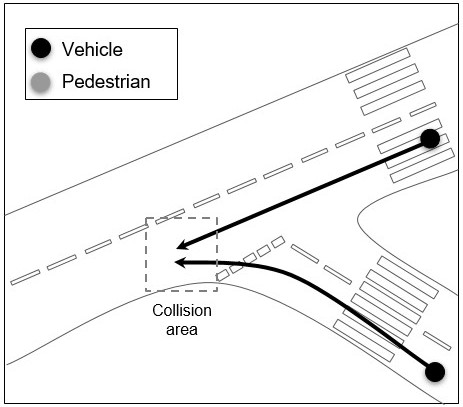
\includegraphics[width=1in]{../document/other/figures/fig3a}


\begin{figure}
    \centering
    \begin{subfigure}
        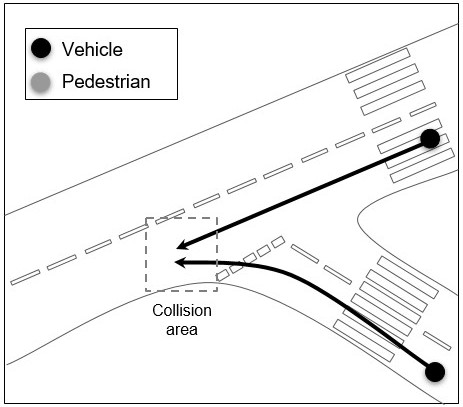
\includegraphics[width=4cm]{../document/other/figures/fig3a}
    \end{subfigure}
    \begin{subfigure}
        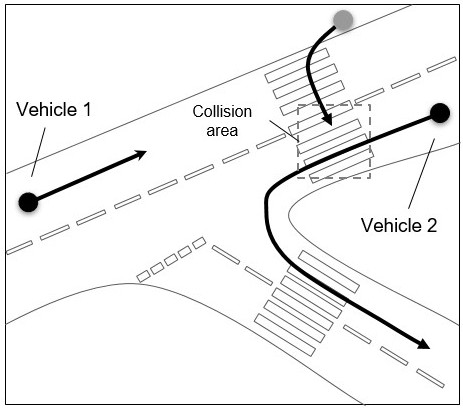
\includegraphics[width=4cm]{../document/other/figures/det_fig3bb}
    \end{subfigure}
    \begin{subfigure}
        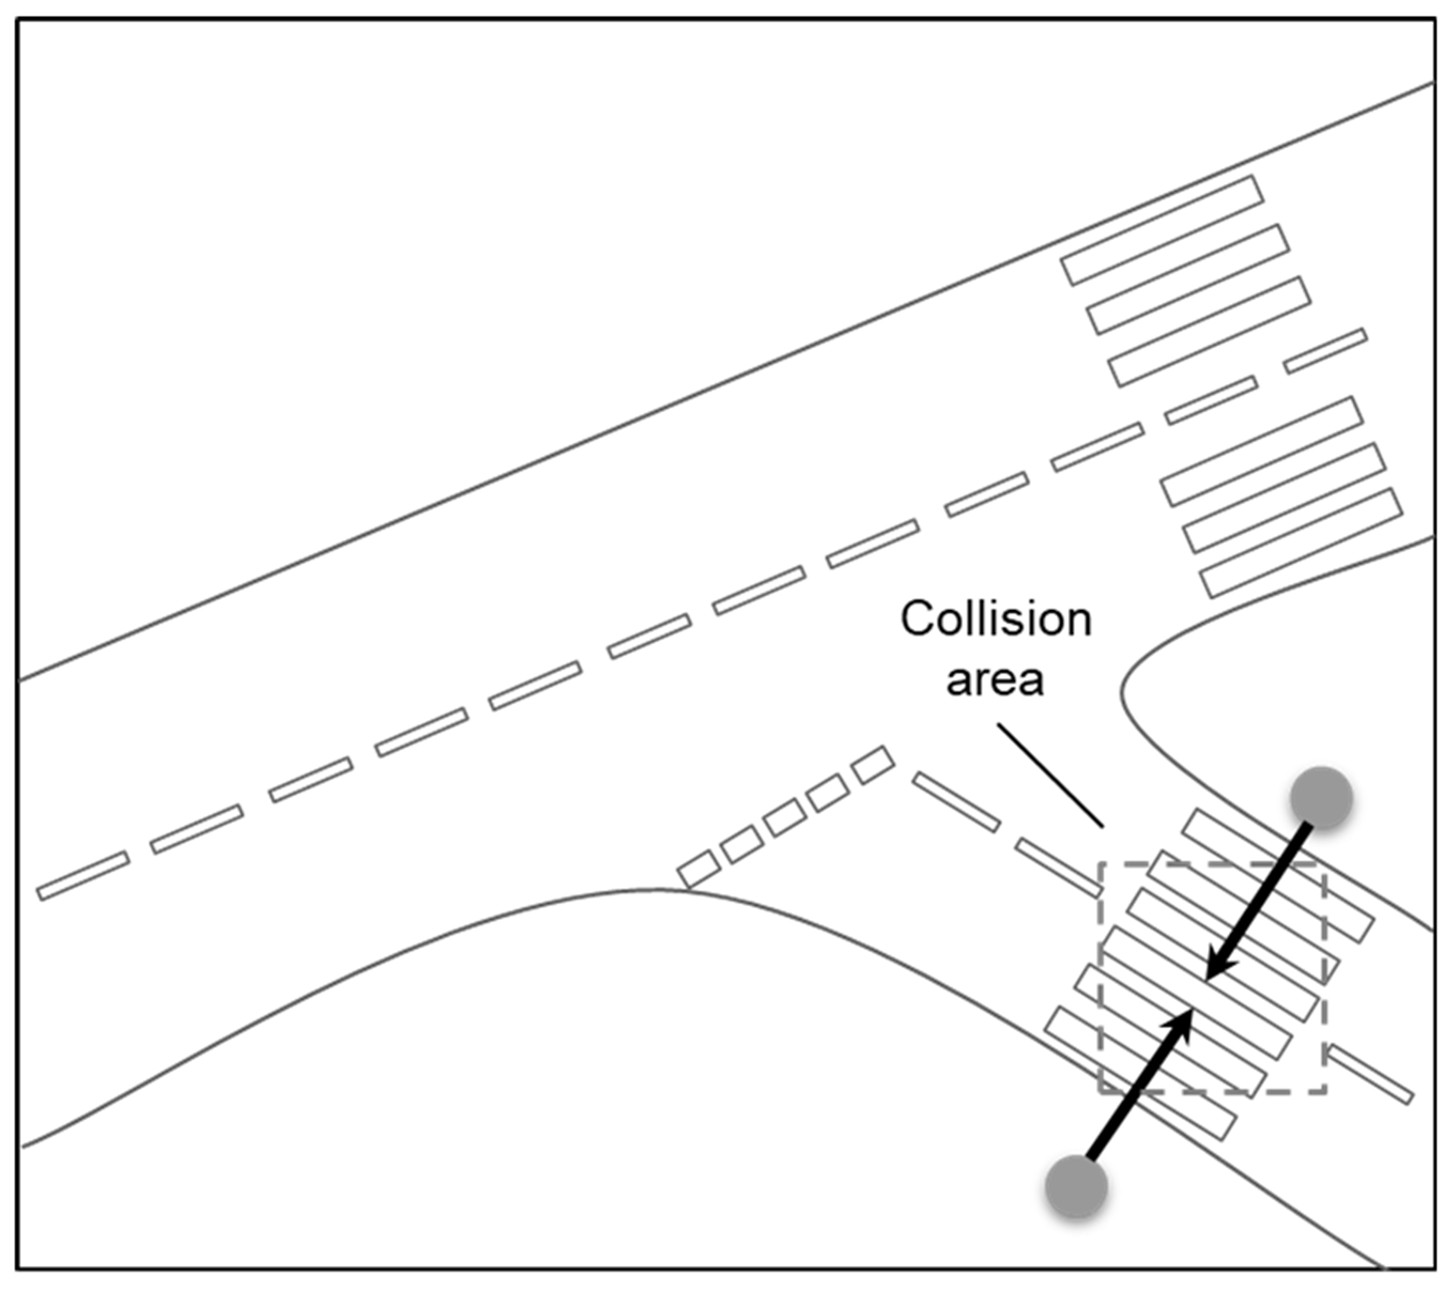
\includegraphics[width=4cm]{../document/other/figures/det_fig3c}
    \end{subfigure}
    \caption{\\Schematic of test scenarios for (a) Tests 1-2, (b) Tests 3-4, (c) Tests 5-6. Descriptions are given in Table~1.}
\end{figure}


\bigskip

\textit{Comment 10: "The size of simulation scenes should be pointed out, especially the boundary of (x, y, z)"}.

Thank you, we agree this would help describe the scene better to the reader. Please see section V.C on page 7 for the additional text:
\begin{quote}
\textit{The map size for the simulation test environment was 354$m$ $\times$ 170$m$. The range of movement of the actors within the environment was up to 70m for vehicles and up to 25m for pedestrians}.
\end{quote}

\bigskip

\textit{Comment 11: "Which vehicle collided with the pedestrian in test 4, please label them in Fig 3"}. 

We agree it would be clearer for the reader if this information was presented. We have added the collision area to Fig.3 (on page 7) indicating where the collision happens and the ID of the vehicles.

\bigskip
\centerline{\rule{13cm}{0.4pt}}
\bigskip

\textbf{Reviewer 2}\\
\textit{Comment 1: "The current paper is a little bit too long and could be shortened. For instance, several definitions in Section II.A could be introduced in a more concise way. Sections II and III could be combined. Sections V and VI could be combined"}.

We agree the paper is a bit long, however if readers are familiar with the definitions it is likely that they will skip over these but it would be prudent to keep them in for the paper to be sufficiently self-contained. We think that section V and VI are already long independently and combining them might become unwieldy. 

We have attempted to reduce the paper size in different areas, please see the diff document. However, as the first reviewer wanted additional material added, including figures, this may have resulted in a net increase in overall manuscript length. 

\bigskip

\textit{Comment 2: "In Section IV, several potential sources of non-determinism are reviewed. Through the case study, the authors should have established a general understanding of the relative significance of each potential source to the overall simulation variance (as least for CARLA). It would be good to comment on the relative significance alongside the review of these sources"}.

We do not consider it feasible to provide a general understanding for the relative significance of each potential source of non-determinism due to the fact that these depend on the verification requirements, the simulation setup, the actual software/hardware configuration used, etc. These factors have been identified in our methodology in section VII. If the reader follows this methodology, then they should be able to discover the principle sources, quantify them and prioritise those which may lead to simulation variance above the permissible level for their use case.

We have illustrated in Table.1 that pedestrian-vehicle collisions result in high simulation variance for our case study, and also the role that resource utilisation plays should be clear to the reader from viewing Fig.4.


\bigskip

\textit{Comment 3: "It would be good if the authors could show the vehicle/pedestrian trajectories of a test case where a large maximum variance occur (such as the trajectories pre and post a collision). This could help the reader better understand the cause of the large trajectory variance"}.

Thank you, this is a great idea and we agree that this would give the reader a better insight into the issue. We have added an X-Y plane data plot showing the high simulation variance that occurs during test 4. In this plot you can see the area that vehicle 2 and the pedestrian collide within and the subsequent path variance (see Fig.5 on page 9). 

\begin{figure}
    \centering
    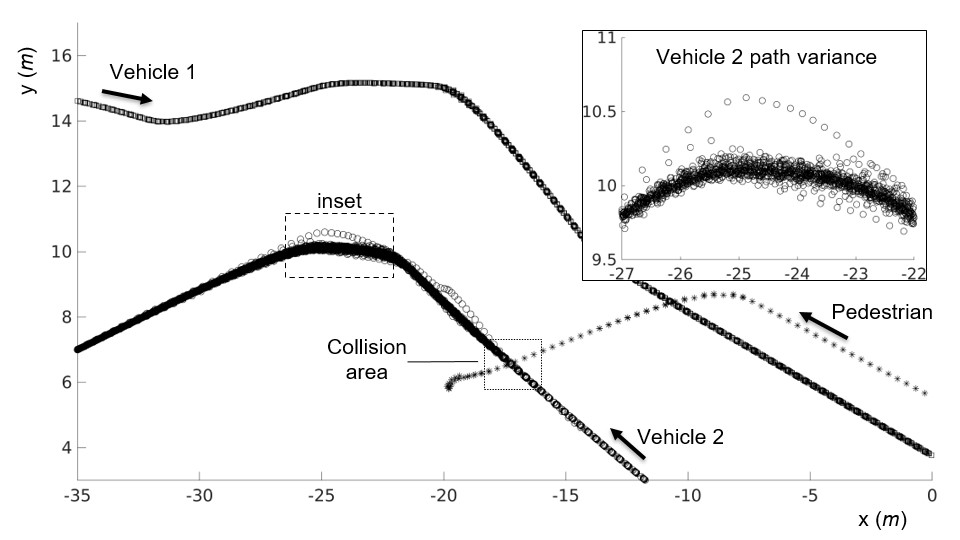
\includegraphics[width=12cm]{../document/other/figures/actor_path_plot.jpg}
    \caption{\\Actor path plot in XY plane for Test 4 with 95\% resource utilisation.}
\end{figure}


This new figure is referenced in the following text (additional in italics):
\begin{quote}
However, all other scenarios involving vehicles or a mixture of actor types do not meet the required tolerance, with some deviation in actor path as large as 59cm. \textit{A plot of actor position in the X-Y plane (plan view, units m) is shown in Fig.5, where the inset shows the divergence of the path of vehicle 2 post-collision with the pedestrian.} Clearly, such a large deviation cannot be acceptable for simulation to be considered a credible verification tool.
\end{quote}

\bigskip

Thank you and the reviewers for your time and consideration to this paper. We hope, given the above changes and explanations, you will consider this manuscript suitable for publishing. 

\bigskip

Sincerely,

\bigskip


\includegraphics[width=1in]{signature.png}

Dr. Greg Chance, PhD, CEng, MInstP

\end{letter}

\end{document}
